\documentclass[10.5pt]{config}
% 本实验报告采用 署名-相同方式共享 4.0 国际许可协议 (CC BY-SA 4.0)
\usepackage{multirow}
\usepackage{wrapfig}
\usepackage{setspace}
\usepackage{titlesec}
\usepackage{ctex}
\usepackage{graphicx} % 用于插入图片
\usepackage{float}    % 用于控制图片位置
\usepackage{makecell}

\titleformat{\subsubsection}[block]  % 设置为块级标题（自动换行）
{\normalfont\bfseries}{\thesubsubsection}{1em}{} 
\titlespacing*{\subsubsection}{1.5em}{3.25ex}{1.5ex}  % 调整缩进：左缩进2em
\setstretch{1.5}

% --- 请在这里填写您的个人信息 ---
\major{} % 专业
\name{}
\partner{} % 签名栏
\stuid{}
\date{}
\lab{}
\grades{}
\course{电工电子学实验}
\instructor{} % 指导老师
\exptype{基础实验} % 实验类型
\expname{叠加定理和等效电源定理验证} % 实验名字


\begin{document}

\makeheader % 首页头部

\section{实验目的和要求}

\begin{enumerate}[label=\arabic*., leftmargin=2em]
    \item 理解掌握叠加定理和等效电源定理。
    \item 验证叠加定理。
    \item 掌握含源一端口网络外特性的测量方法。
    \item 验证等效电源定理。
\end{enumerate}

\section{实验内容和原理}


\subsection{实验原理}

\subsubsection*{1.1 叠加定理}

线性电路中，若干独立电源共同作用下的任意支路上的电流或电压等于各个独立电源单独作用时分别在该支路所产生的电流或电压的代数和。当其中某个独立电源单独作用时，其余的独立电源被除去（电路中电压源所在位置予以短路，电流源所在位置予以开路）。

\subsubsection*{1.2 等效电源定理}

等效电源定理包括戴维宁等效定理和诺顿等效定理。

一个线性有源二端网络可用一个电压源和一个电阻串联的电路来等效，该电压源的电压等于此有源二端网络的开路电压 $U_{\mathrm{OC}}$，串联电阻等于此有源二端网络除去独立电源后在其端口处的等效电阻 $R_0$。此即为戴维宁定理，而这个电压源和电阻串联的等效电路称为戴维宁等效电路。

\begin{figure}[H]
    \centering
    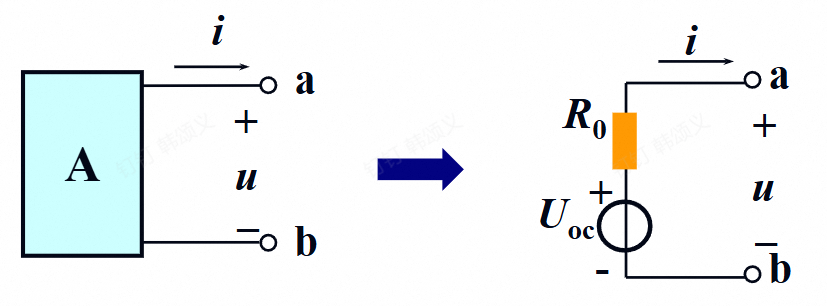
\includegraphics[width=0.55\textwidth]{figures/daiweining.png}
    \caption{戴维宁等效电路}
    \label{fig:daiweining}
\end{figure}

一个线性有源二端网络可用一个电流源和一个电阻并联的电路来等效，该电流源的电流等于此有源二端网络的短路电流 $I_{\mathrm{SC}}$，并联电阻等于此有源二端网络除去独立电源后在其端口处的等效电阻 $R_0$。此即为诺顿定理，而这个电流源和电阻并联的等效电路称为诺顿等效电路。

\begin{figure}[H]
    \centering
    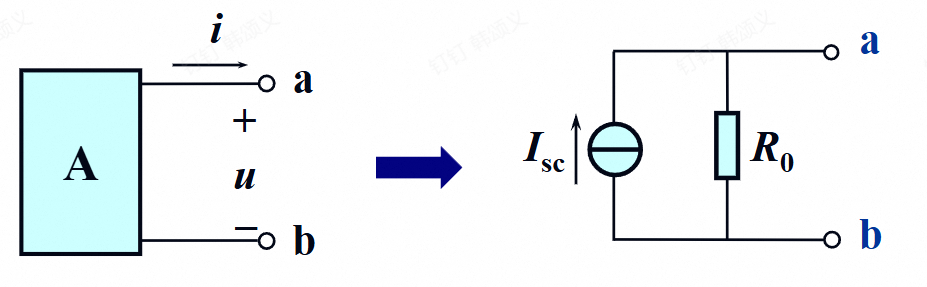
\includegraphics[width=0.55\textwidth]{figures/nuodun.png}
    \caption{诺顿等效电路}
    \label{fig:nuodun}
\end{figure}

戴维宁等效电路与诺顿等效电路均与原始线性有源二端网络等效，而等效之后的戴维宁等效电路与诺顿等效电路之间也相互等效。戴维宁等效电路与诺顿等效电路的参数测量实际可归结为原始线性有源二端网络的开路电压 $U_{\mathrm{OC}}$、短路电流 $I_{\mathrm{SC}}$ 以及等效电阻 $R_0$ 的测量。



\section{主要仪器设备}
\begin{enumerate}[label=\arabic*., leftmargin=2em]
    \item 电工电子综合实验台。
    \item 稳压电源。
    \item 电阻元件，十进制电阻箱。
    \item 数字式万用表。

\end{enumerate}

\section{操作方法和实验步骤}

\subsection*{1. 验证叠加定理}
按图3所示连接实验电路，其中 $U_S = 9\,\mathrm{V}$，$I_S = 10\,\mathrm{mA}$。采用直流电压表和直流电流表，选择合适的量程，分别测量电压源 $U_S$ 单独作用、电流源 $I_S$ 单独作用，以及电压源 $U_S$ 与电流源 $I_S$ 共同作用时，两个 $510\,\Omega$ 电阻上的电压 $U_1$、$U_3$，流经 $510\,\Omega$ 电阻的电流 $I_2$（注意电压、电流的参考方向），将测量数据填入表1中。

\begin{figure}[H]
    \centering
    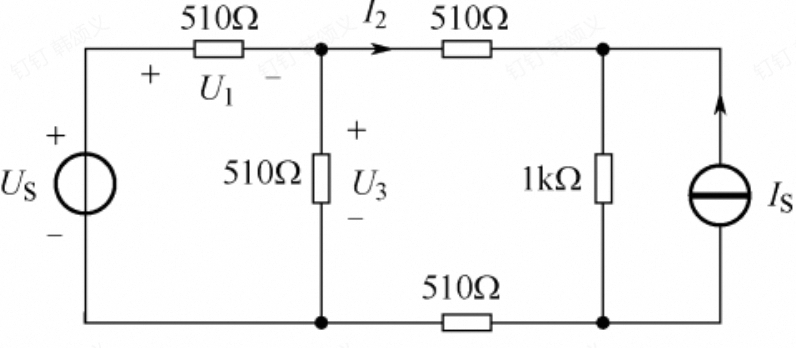
\includegraphics[width=0.6\textwidth]{figures/diejia.png}
    \caption{验证叠加定理电路图}
    \label{fig:diejia}
\end{figure}

\subsection*{2. 验证等效电源定理}

\subsubsection*{(1)}
按图4所示连接实验电路，改变AB端口上外接电阻的阻値 $R$，测量图中所示含源二端网络的外特性，记录电阻値 $R$、端口电压 $U_{\mathrm{AB}}$ 以及端口电流 $I_R$，将测量数据填入表2中。

\begin{figure}[H]
    \centering
    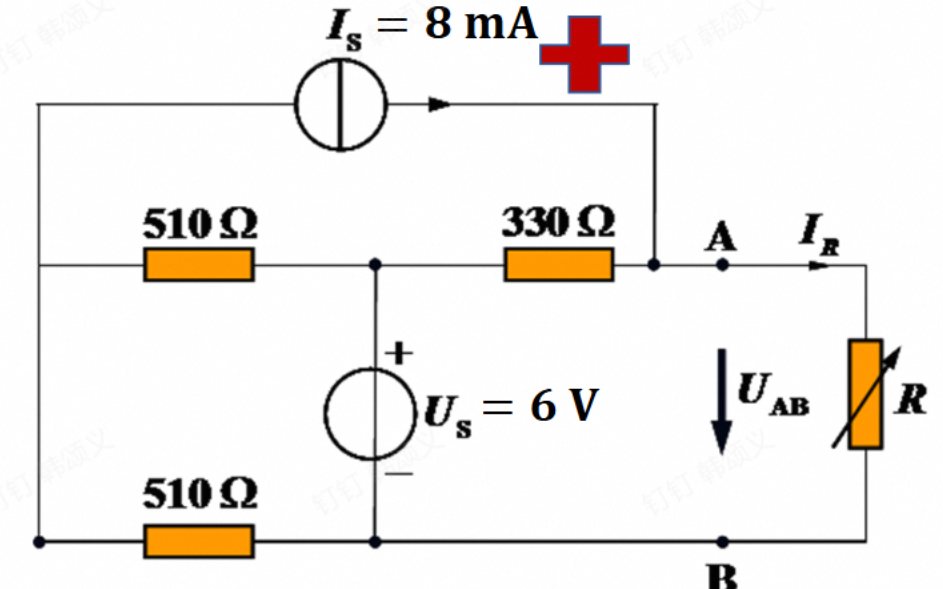
\includegraphics[width=0.6\textwidth]{figures/dengxiao.png}
    \caption{验证等效电源定理电路图}
    \label{fig:dengxiao}
\end{figure}

\subsubsection*{(2)}
将图4中独立电压源、独立电流源除去（电路中电压源位置予以短路，电流源位置予以开路），同时不接外部电阻，用万用表测量 A、B 间电阻即此含源二端网络的等效电阻 $R_0 = 336.0\Omega$。

\subsubsection*{(3)}
依据以上所测量的开路电压 $U_{\mathrm{OC}}$ 与等效电阻 $R_0$ 构造戴维宁等效电路，选择和表2中相同的电阻 $R$，测量此戴维宁等效电路的外特性，将测量数据填入表3中。

\subsubsection*{(4)}
依据以上所测量的短路电流 $I_{\mathrm{SC}}$ 与等效电阻 $R_0$ 构造诺顿等效电路，选择和表2中相同的电阻 $R$，测量此诺顿等效电路的外特性，将测量数据填入表4中。


\section{实验数据记录和处理}
\subsection{数据记录}

% 表5.3-1 验证叠加定理
\begin{table}[H]
    \centering
    \small
    \begin{tabular}{|c|c|c|c|}
        \hline
         & $U_1/\mathrm{V}$ & $I_2/\mathrm{mA}$ & $U_3/\mathrm{V}$ \\
        \hline
        电压源 $U_S$ 单独作用 &5.013 & 2.03&3.989 \\
        \hline
        电流源 $I_S$ 单独作用 & -1.131& -4.48& 1.130\\
        \hline
        以上两者叠加结果（计算）  & 3.882& -2.45& 5.119\\
        \hline
        电压源 $U_S$ 与电流源 $I_S$ 共同作用 & 3.883& -2.50&5.119 \\
        \hline
    \end{tabular}
    \caption{验证叠加定理}
    \label{tab:superposition}
\end{table}

0.6
% 表5.3-2 验证等效电源定理
\begin{table}[H]
    \centering
    \small
    \begin{tabular}{|c|c|c|c|c|c|c|}
        \hline
        $R/\Omega$ & 0 & 100 & 200 & 500 & 1200 & $\infty$ \\
        \hline
        $U_{\mathrm{AB}}/\mathrm{V}$ & /& 1.995& 3.241& 5.196&6.78 & 8.68\\
        \hline
        $I_R/\mathrm{mA}$ &25.83 &19.85 &16.21 &10.38 &5.60 &/ \\
        \hline
        测量说明 & 短路电流 $I_{\mathrm{SC}}$ & & & & & 开路电压 $U_{\mathrm{OC}}$ \\
        \hline
    \end{tabular}
    \caption{验证等效电源定理}
    \label{tab:thevenin}
\end{table}

% 表5.3-3 戴维宁等效电路外特性测量
\begin{table}[H]
    \centering
    \small
    \begin{tabular}{|c|c|c|c|c|c|c|}
        \hline
        $R/\Omega$ & 0 & 100 & 200 & 500 & 1200 & $\infty$ \\
        \hline
        $U_{\mathrm{AB}}/\mathrm{V}$ & /&1.959 &3.183 &5.139& 6.72&8.70 \\
        \hline
        $I_R/\mathrm{mA}$ &25.28 &19.55 &16.04&10.23 &5.57 &/ \\
        \hline
        测量说明 & 短路电流 $I_{\mathrm{SC}}$ & & &  & &  开路电压 $U_{\mathrm{OC}}$ \\
        \hline
    \end{tabular}
    \caption{戴维宁等效电路外特性测量}
    \label{tab:thevenin_equiv}
\end{table}

% 表5.3-4 诺顿等效电路外特性测量
\begin{table}[H]
    \centering
    \small
    \begin{tabular}{|c|c|c|c|c|c|c|}
        \hline
        $R/\Omega$ & 0 & 100 & 200 & 500 & 1200 & $\infty$ \\
        \hline
        $U_{\mathrm{AB}}/\mathrm{V}$ & /&1.979 &3.215 &5.190 &6.80 &8.74 \\
        \hline
        $I_R/\mathrm{mA}$ &25.58 & 19.81&16.19 &10.40 &5.64&/ \\
        \hline
        测量说明 & 短路电流 $I_{\mathrm{SC}}$ & & & & & 开路电压 $U_{\mathrm{OC}}$ \\
        \hline
    \end{tabular}
    \caption{诺顿等效电路外特性测量}
    \label{tab:norton_equiv}
\end{table}


\subsection{数据处理}

对表2、表3、表4中各组测量数据分别进行线性拟合，拟合方程均为 $U_{\mathrm{AB}} = k \cdot I_R + b$的形式。

\begin{figure}[H]
    \centering
    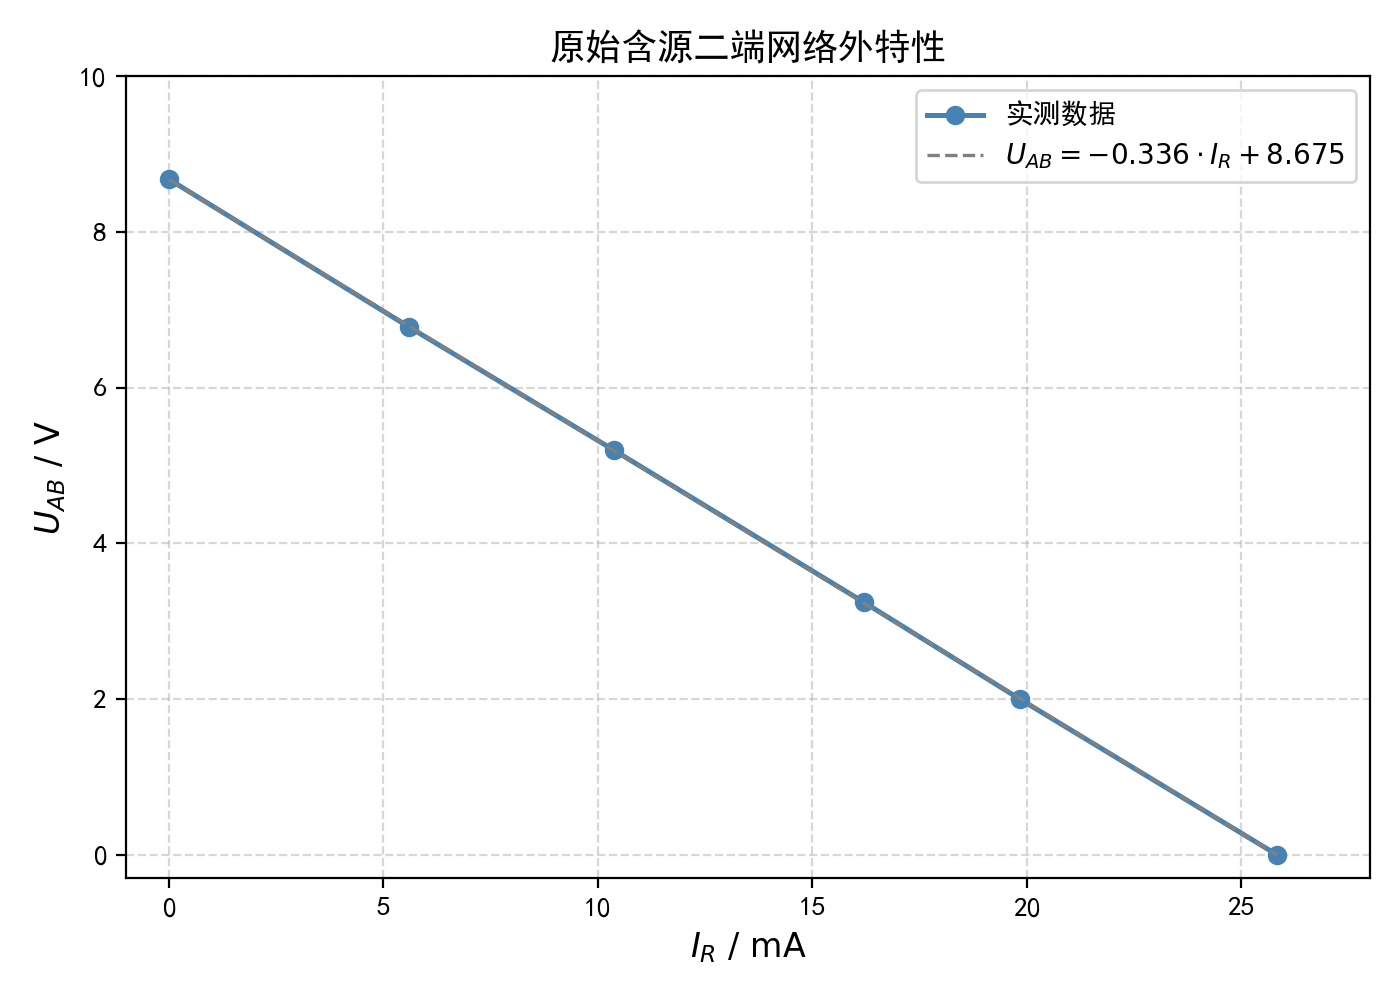
\includegraphics[width=0.4\textwidth]{figures/orig_char.png}
    \caption{原始含源二端网络外特性曲线}
    \label{fig:orig_char}
\end{figure}

\begin{figure}[H]
    \centering
    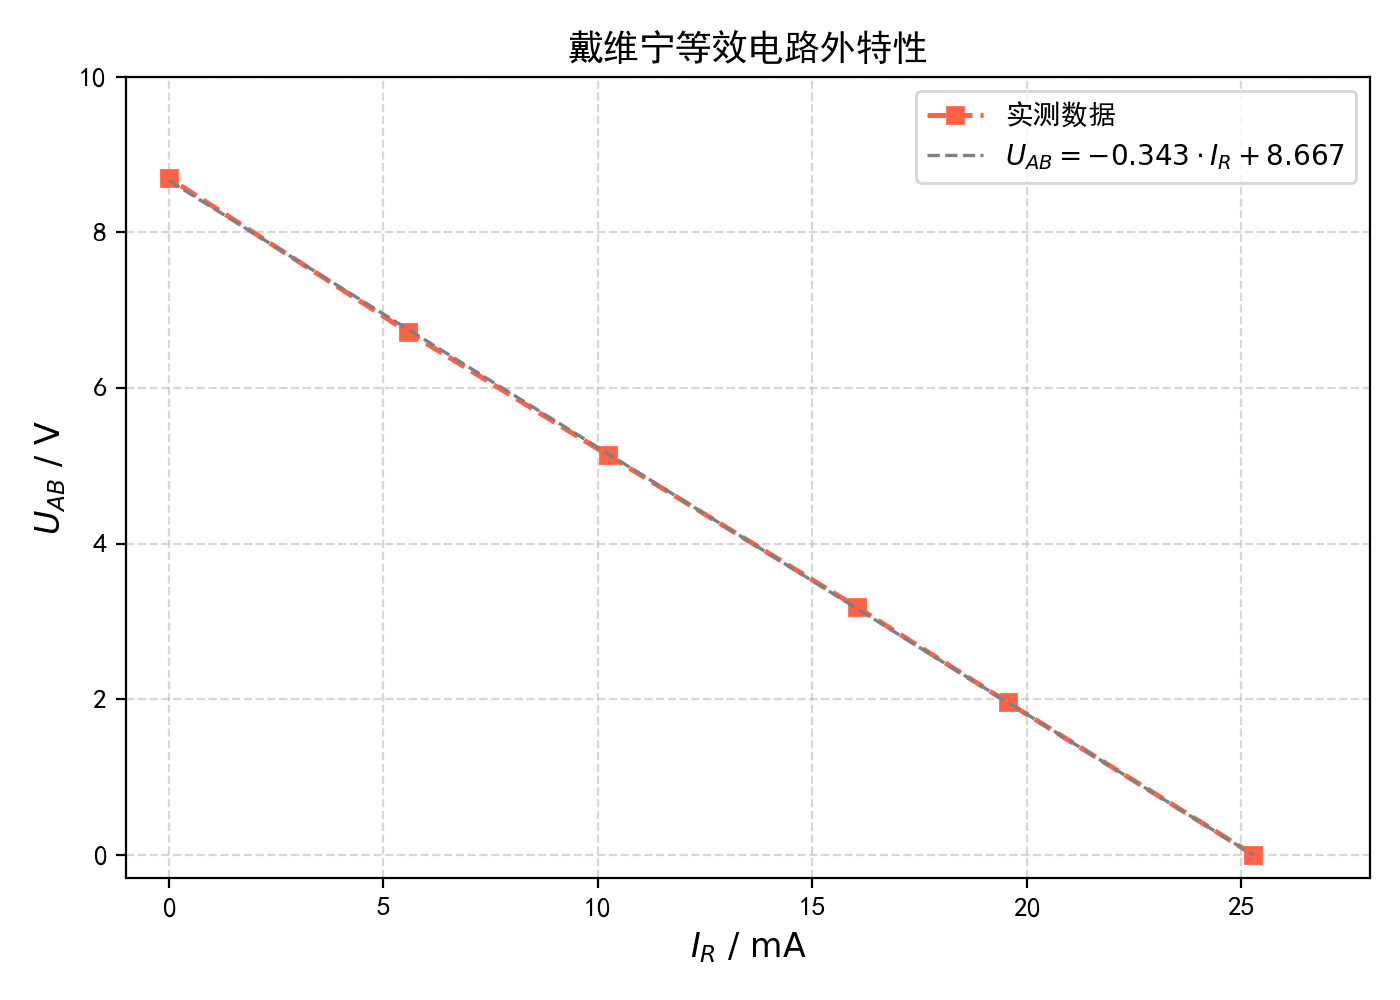
\includegraphics[width=0.4\textwidth]{figures/thev_char.png}
    \caption{戴维宁等效电路外特性曲线}
    \label{fig:thev_char}
\end{figure}

\begin{figure}[H]
    \centering
    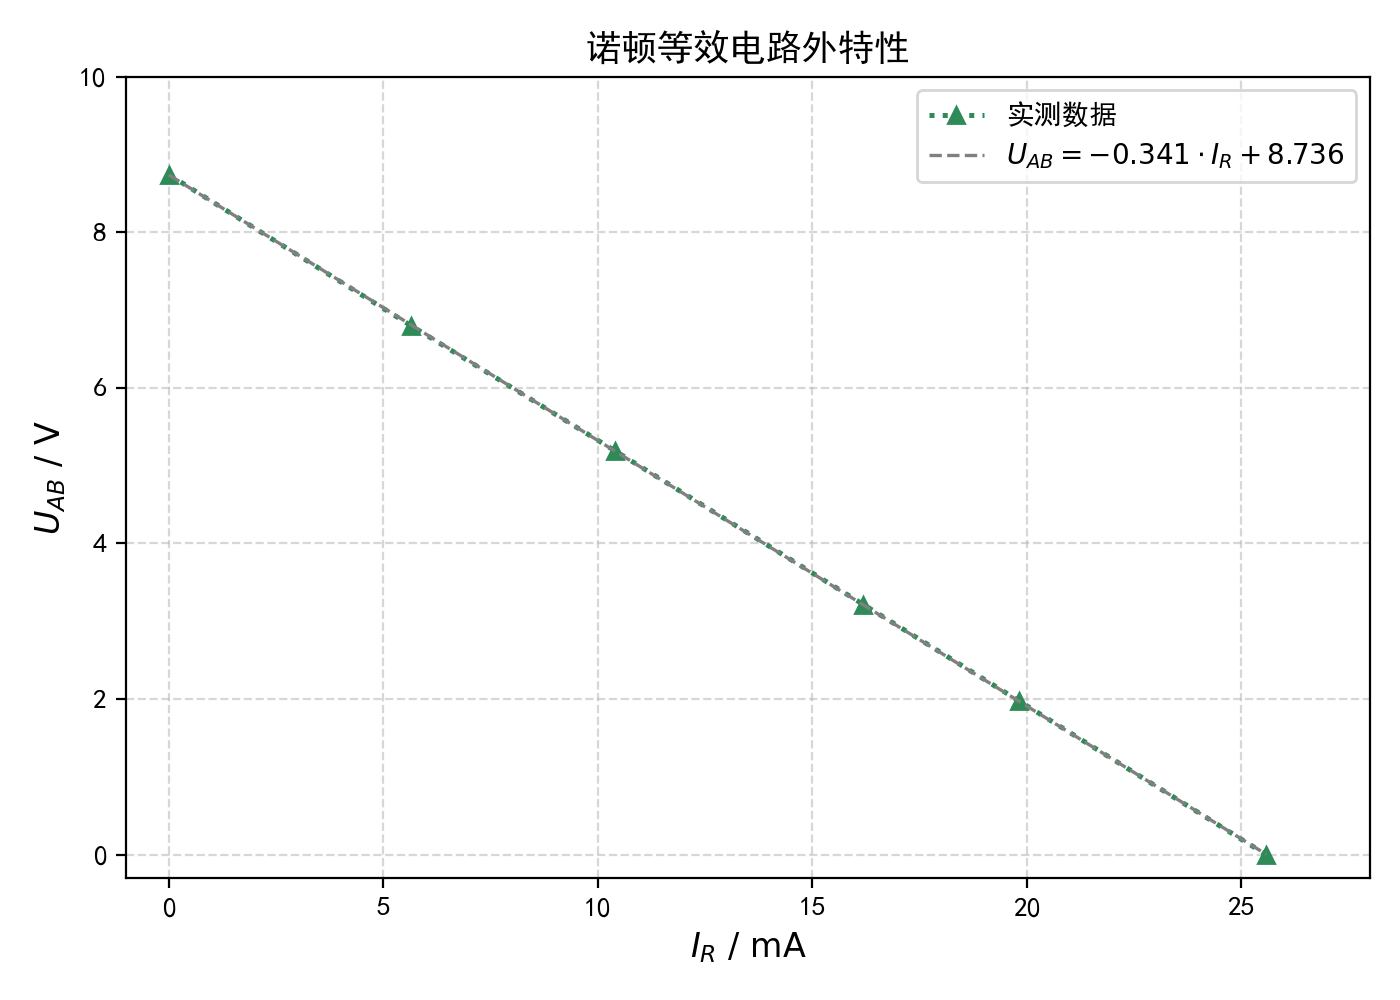
\includegraphics[width=0.4\textwidth]{figures/nort_char.png}
    \caption{诺顿等效电路外特性曲线}
    \label{fig:nort_char}
\end{figure}
\section*{六、实验结果与分析}

\subsection*{1. 叠加定理验证}

根据表1的数据，将电压源 $U_S$ 单独作用与电流源 $I_S$ 单独作用时的测量値代数叠加，得：
\begin{equation*}
    U_1^{\text{叠加}} = 5.013 + (-1.131) = 3.882\ \mathrm{V},\quad
    I_2^{\text{叠加}} = 2.03 + (-4.48) = -2.45\ \mathrm{mA},\quad
    U_3^{\text{叠加}} = 3.989 + 1.130 = 5.119\ \mathrm{V}
\end{equation*}
将叠加计算値与实测共同作用値（$U_1=3.883\ \mathrm{V}$、$I_2=-2.50\ \mathrm{mA}$、$U_3=5.119\ \mathrm{V}$）对比：
\begin{itemize}
    \item $U_1$：相对误差 $0.03\%$，吸合良好；
    \item $I_2$：相对误差 $2.0\%$，在仪表精度范围内；
    \item $U_3$：相对误差 $0\%$，吸合完美。
\end{itemize}
三组测量量的叠加计算値与实测吹合度均優于 $98\%$，验证了线性电路中叠加定理成立。存在小误差主要来源于电表内阻的分流分压以及读数误差。

\subsection*{2. 等效电源定理验证}

\textbf{（1）含源二端网络参数测量：}
由表2实测得开路电压 $U_{\mathrm{OC}} = 8.68\ \mathrm{V}$、短路电流 $I_{\mathrm{SC}} = 25.83\ \mathrm{mA}$，直接测量等效内阻 $R_0 = 336.0\ \Omega$。由外特性拟合直线验证：
\begin{equation*}
    R_0 = \frac{U_{\mathrm{OC}}}{I_{\mathrm{SC}}} = \frac{8.68\ \mathrm{V}}{25.83\ \mathrm{mA}} \approx 336.0\ \Omega
\end{equation*}
与直接测量値完全吹合。

\textbf{（2）三种电路外特性对比：}
如图\ref{fig:orig_char}、图\ref{fig:thev_char}、图\ref{fig:nort_char}所示，原始含源二端网络、戴维宁等效电路、诺顿等效电路的外特性曲线高度重合。三种电路关键参数对比如下：
\begin{itemize}
    \item 开路电压 $U_{\mathrm{OC}}$：$8.68\ \mathrm{V}$、$8.70\ \mathrm{V}$、$8.74\ \mathrm{V}$，最大偏差 $0.7\%$；
    \item 短路电流 $I_{\mathrm{SC}}$：$25.83\ \mathrm{mA}$、$25.28\ \mathrm{mA}$、$25.58\ \mathrm{mA}$，最大偏差 $2.1\%$。
\end{itemize}
三者外特性高度重合，充分验证了戴维宁定理与诺顿定理的正确性。实验中存在的小量偏差主要来自电表内阻的影响、等效电路流的元件容差以及搭建等效电路时电阻算的读数误差。

\section*{七、讨论、心得}

本次实验通过叠加定理和等效电源定理的验证，加深了对线性电路分析方法的理解。实验中需特别注意各电压、电流的参考方向，当某一电源单独作用时其贡献值可能为负，这是叠加定理中容易出错之处。等效电源定理部分，通过分别构造戴维宁和诺顿等效电路并测量其外特性，直观体会到两种等效电路与原始网络的等价性。实验误差主要来自电表内阻的影响和电阻箱的读数误差，整体结果在合理范围内，实验达到了预期目的。

\end{document}



